%----------------------------------------------------------------------------
\clearpage\section{Using this \LaTeX{} template}\label{app:latex}
%----------------------------------------------------------------------------
% TODO Delete this appendix (the \input in content/appendices.tex) before submission.
This appendix uses every package that \texttt{include/packages.tex} loads, every theorem-like environment, and every tagged list, on one running example: an issuer revokes verifiable credentials in a shared registry.
Copy what you need from the source, \texttt{content/appendix-latex.tex}.
\Cref{tab:package-index} at the end lists each package and where it is shown.

%----------------------------------------------------------------------------
\subsection{Todo notes (todonotes)}\label{app:latex:todo}
A margin note sits next to the line it refers to.\todo{A margin note.}
The margins are narrow, so prefer inline notes:
\todo[inline]{An inline note: a block across the text width.}
\todoinline{The same, with the \texttt{\textbackslash todoinline} shortcut.}
\todo[inline, color=green!25, author=Supervisor]{A note with an author and its own color, for review comments.}
\missingfigure{A placeholder for a figure that does not exist yet.}

All notes are collected in the list of todos after the table of contents.
To hide them in the submitted version, load todonotes with the \texttt{disable} option and remove \texttt{\textbackslash listoftodos} from \texttt{thesis.tex}.

%----------------------------------------------------------------------------
\subsection{Acronyms (acro)}\label{app:latex:acro}
The first use expands: \ac{vc}. Later uses stay short: \ac{vc}. The plural: \acp{vc}.
Short and long forms on demand: \acs{zkp}, \acl{zkp}.
Declare acronyms in \texttt{content/acronyms.tex}; the list of acronyms is printed after the list of tables.

%----------------------------------------------------------------------------
\subsection{Citations, links and icons (natbib, hyperref, bookmark, orcidlink, fontawesome5)}\label{app:latex:cite}
Numeric citations are sorted and compressed~\cite{w3c2025vcdm,lamport1978time}.
\texttt{\textbackslash citet} names the author: \citet{lamport1978time} introduced logical clocks.
\texttt{\textbackslash citep} brackets the reference~\citep{lamport1978time}.

Links: \url{https://github.com/ftsrg} prints the address, \href{https://ftsrg.mit.bme.hu}{the research group} hides it.
The PDF bookmarks in the viewer's sidebar come from hyperref and bookmark.
Icons: \faGithub~source code, \faFilePdf~paper, \faEnvelope~contact. Author ORCID: \orcidlink{0000-0000-0000-0000}.

%----------------------------------------------------------------------------
\subsection{Cross-references (cleveref)}\label{app:latex:cref}
Use \texttt{\textbackslash cref} for every reference, so the type name comes for free, and \texttt{\textbackslash Cref} at the start of a sentence:
\cref{fig:latex:tikz,fig:latex:svg}, \cref{tab:latex:booktabs}, \cref{alg:latex:revoke}, \cref{lst:latex:verify}, \cref{eq:latex:window}, \cref{app:latex:theorems}.
Ranges compress: \cref{eq:latex:window,eq:latex:fresh,eq:latex:valid}.
\Cref{app:latex:theorems,app:latex:tags} reference every theorem-like environment and tagged list.
Label prefixes are listed in \texttt{include/preamble.tex}.

%----------------------------------------------------------------------------
\subsection{Mathematics and theorem-like environments (amsmath, amssymb, ntheorem)}\label{app:latex:theorems}
A numbered equation:
\begin{equation}\label{eq:latex:window}
  \mathit{valid}(c, t) \iff t \in [t_\mathrm{issue}(c), t_\mathrm{exp}(c)) \land c \notin R_t .
\end{equation}
Aligned equations, each with its own number:
\begin{align}
  R_{t+1} &= R_t \cup \{ c \} \label{eq:latex:fresh}\\
  \mathit{valid}(c, t+1) &\implies \mathit{valid}(c, t) \label{eq:latex:valid}
\end{align}
Symbols from amssymb: $\mathbb{N}$, $\mathcal{R}$, $\nexists$, $\varnothing$.

Every theorem-like environment, in a typical order.
Definitions and examples have their own counters; the rest share the theorem counter.
\begin{definition}[Revocation registry]\label{def:latex:registry}
A \emph{revocation registry} is a set $R_t$ of revoked credential identifiers at time $t \in \mathbb{N}$.
\end{definition}
\begin{notation}\label{not:latex:issuer}
$I(c)$ denotes the issuer of credential $c$.
\end{notation}
\begin{example}\label{ex:latex:registry}
A university revokes a diploma credential $c$ at $t=5$, so $c \in R_5$.
\end{example}
\begin{invariant}\label{inv:latex:monotone}
The registry only grows: $R_t \subseteq R_{t+1}$ for every $t$.
\end{invariant}
\begin{property}[Revocation is final]\label{prty:latex:final}
If $c \in R_t$, then $\mathit{valid}(c, t')$ is false for every $t' \geq t$.
\end{property}
\begin{lemma}\label{lem:latex:step}
If $\mathit{valid}(c, t+1)$, then $\mathit{valid}(c, t)$, by \cref{eq:latex:valid}.
\end{lemma}
\begin{proof}
By \cref{inv:latex:monotone}, $c \notin R_{t+1}$ implies $c \notin R_t$.
\end{proof}
\begin{theorem}[Finality]\label{thm:latex:finality}
\Cref{prty:latex:final} holds for every registry that satisfies \cref{inv:latex:monotone}.
\end{theorem}
\begin{proof}
Induction on $t' - t$ with \cref{lem:latex:step}.
\end{proof}
\begin{corollary}\label{cor:latex:noresurrect}
A revoked credential is never valid again.
\end{corollary}
\begin{proposition}\label{prop:latex:size}
After $n$ revocations, $|R_t| = n$.
\end{proposition}
\begin{claim}\label{claim:latex:append}
An append-only log implements $R_t$.
\end{claim}
\begin{remark}\label{rem:latex:expiry}
Expiry is not revocation: an expired credential is not in $R_t$.
\end{remark}
References: \cref{def:latex:registry}, \cref{not:latex:issuer}, \cref{ex:latex:registry}, \cref{inv:latex:monotone}, \cref{prty:latex:final}, \cref{lem:latex:step}, \cref{thm:latex:finality}, \cref{cor:latex:noresurrect}, \cref{prop:latex:size}, \cref{claim:latex:append}, \cref{rem:latex:expiry}.

%----------------------------------------------------------------------------
\subsection{Tagged lists and other lists (enumitem)}\label{app:latex:tags}
Tagged lists give short, stable names to the things a paper argues about.
Add a new kind with one \texttt{\textbackslash NewTagList} line in \texttt{include/preamble.tex}.
\begin{contributions}
  \item\label{c:latex:model} A formal model of revocation registries.
  \item\label{c:latex:impl} An implementation on a permissioned ledger.
\end{contributions}
\begin{rqlist}
  \item\label{rq:latex:latency} How long does a revocation take to become visible?
\end{rqlist}
\begin{requirements}
  \item\label{req:latex:offline} Verifiers can check revocation status offline.
\end{requirements}
\begin{threats}
  \item\label{thr:latex:replay} A holder replays a credential after its revocation.
\end{threats}
\begin{assumptions}
  \item\label{asm:latex:clock} Participants' clocks drift by at most $\delta$.
\end{assumptions}
\begin{guarantees}
  \item\label{g:latex:detect} Under \cref{asm:latex:clock}, every replay in \cref{thr:latex:replay} is rejected within $\delta$.
\end{guarantees}
\begin{limitations}
  \item\label{lim:latex:liveness} The registry cannot force an issuer to revoke.
\end{limitations}
References: \cref{c:latex:model,c:latex:impl}, \cref{rq:latex:latency}, \cref{req:latex:offline}, \cref{thr:latex:replay}, \cref{asm:latex:clock}, \cref{g:latex:detect}, \cref{lim:latex:liveness}.

Inline lists: the protocol has three roles, \begin{enumerate*}[label=(\roman*)] \item issuer, \item holder, and \item verifier. \end{enumerate*}
Compact lists:
\begin{itemize}[noitemsep]
  \item no extra space between items,
  \item set per list with enumitem options.
\end{itemize}

%----------------------------------------------------------------------------
\subsection{Figures (graphicx, svg, tikz, pgfplots, subcaption, wrapfig, rotating, placeins)}\label{app:latex:figures}
\Cref{fig:latex:tikz} is drawn in TikZ, so it uses the document's fonts and scales without blurring.
\begin{figure}[!ht]
  \centering
  \begin{tikzpicture}[node distance=8mm and 18mm,
      role/.style={draw, rounded corners, fill=blue!8, minimum width=24mm, minimum height=9mm, font=\small},
      store/.style={draw, cylinder, shape border rotate=90, aspect=0.25, fill=gray!15, minimum width=18mm, minimum height=12mm, font=\small}]
    \node[role] (issuer) {Issuer};
    \node[role, right=of issuer] (holder) {Holder};
    \node[role, right=of holder] (verifier) {Verifier};
    \node[store, below=of holder] (reg) {Registry};
    \draw[-Stealth] (issuer) -- node[above, font=\footnotesize]{issue} (holder);
    \draw[-Stealth] (holder) -- node[above, font=\footnotesize]{present} (verifier);
    \draw[-Stealth, dashed] (issuer) |- node[pos=0.75, below, font=\footnotesize]{revoke} (reg);
    \draw[-Stealth, dashed] (verifier) |- node[pos=0.75, below, font=\footnotesize]{check} (reg);
  \end{tikzpicture}
  \caption{A TikZ diagram: roles and the revocation registry.}\label{fig:latex:tikz}
\end{figure}

\Cref{fig:latex:svg} is an SVG file included with \texttt{\textbackslash includesvg}. Overleaf converts it with Inkscape; local builds need \texttt{-shell-escape}.
Export draw.io and Inkscape drawings as SVG and include them this way, so the text stays sharp.
\begin{figure}[!ht]
  \centering
  \includesvg[width=0.35\linewidth]{figures/example}
  \caption{An SVG figure.}\label{fig:latex:svg}
\end{figure}

\Cref{fig:latex:sub} places two subfigures side by side; each has its own label, \cref{fig:latex:sub-a} and \cref{fig:latex:sub-b}.
\begin{figure}[!ht]
  \centering
  \begin{subfigure}[b]{0.45\linewidth}
    \centering
    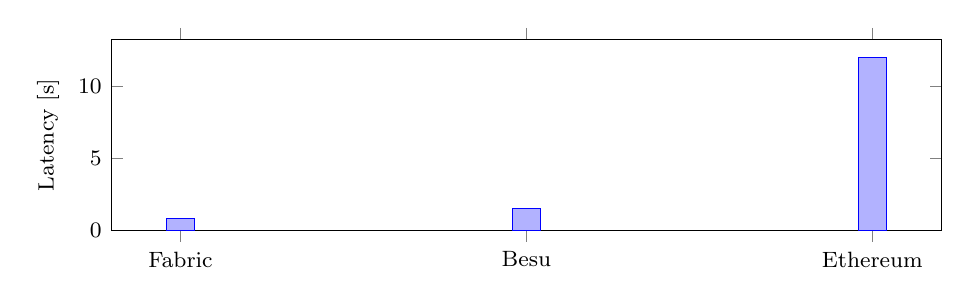
\begin{tikzpicture}
      \begin{axis}[ybar, width=\linewidth, height=40mm, symbolic x coords={Fabric, Besu, Ethereum}, xtick=data, ylabel={Latency [s]}, ymin=0, font=\footnotesize]
        \addplot coordinates {(Fabric,0.8) (Besu,1.5) (Ethereum,12)};
      \end{axis}
    \end{tikzpicture}
    \caption{A pgfplots bar chart.}\label{fig:latex:sub-a}
  \end{subfigure}\hfill
  \begin{subfigure}[b]{0.45\linewidth}
    \centering
    
\includegraphics[width=0.6\linewidth]{figures/bme_logo}
    \caption{A PDF image via graphicx.}\label{fig:latex:sub-b}
  \end{subfigure}
  \caption{Subfigures with subcaption.}\label{fig:latex:sub}
\end{figure}

\begin{wrapfigure}{r}{0.3\linewidth}
  \centering
  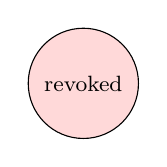
\begin{tikzpicture}
    \node[draw, circle, fill=red!15, minimum size=14mm, font=\footnotesize] {revoked};
  \end{tikzpicture}
  \caption{A wrapped figure.}\label{fig:latex:wrap}
\end{wrapfigure}
Text flows around \cref{fig:latex:wrap}, which wrapfig places at the right margin.
Use it for small figures only, and never next to a list or a section heading, where wrapfig breaks.
The paragraph needs enough lines to wrap around the figure, so this one goes on for a few more sentences.
A revoked credential stays revoked; the registry never forgets.
Verifiers check the registry before accepting a presentation.

\FloatBarrier
The \texttt{\textbackslash FloatBarrier} command from placeins above this line keeps every earlier figure before it.
Put one before a section whose text must not be preceded by stray floats.

%----------------------------------------------------------------------------
\subsection{Colored boxes (tcolorbox)}\label{app:latex:boxes}
\begin{infobox}[Information]
  A general-purpose box for background facts.
\end{infobox}
\begin{warnbox}[Threat model caveat]
  A box for warnings and limitations.
\end{warnbox}
\begin{keybox}[Key insight]
  The \texttt{theo} style; any color works: \texttt{\textbackslash begin\{tcolorbox\}[theo=red, title=...]}.
\end{keybox}

%----------------------------------------------------------------------------
\subsection{Tables (booktabs, array, tabularx, xltabular, multirow, makecell, rotating)}\label{app:latex:tables}
\Cref{tab:latex:booktabs} uses booktabs rules, a bold first column defined with array's \texttt{>\{\textbackslash bfseries\}}, a stretching tabularx column, multirow, makecell, and a colored row from xcolor.
\begin{table}[!ht]
  \centering
  \caption{A booktabs table with tabularx, multirow, makecell and a colored row.}\label{tab:latex:booktabs}
  \begin{tabularx}{\linewidth}{>{\bfseries}l X c}
    \toprule
    Platform & Revocation mechanism & \makecell{Latency\\{[s]}} \\
    \midrule
    \multirow{2}{*}{Fabric} & Chaincode-managed registry & 0.8 \\
     & Private data collections & 1.1 \\
    \rowcolor{gray!15}
    Ethereum & Smart-contract status list & 12 \\
    \bottomrule
  \end{tabularx}
\end{table}

\Cref{tab:latex:long} is an xltabular: a tabularx that breaks across pages and repeats its header.
\begin{xltabular}{\linewidth}{l X}
  \caption{A table that may break across pages.}\label{tab:latex:long}\\
  \toprule
  \textbf{Package} & \textbf{Purpose} \\
  \midrule
  \endfirsthead
  \toprule
  \textbf{Package} & \textbf{Purpose} \\
  \midrule
  \endhead
  todonotes & Visible notes while drafting \\
  acro & Acronyms expanded on first use \\
  tcolorbox & Colored boxes \\
  \bottomrule
\end{xltabular}

\Cref{tab:latex:sideways} is too wide for the page, so rotating turns it sideways onto its own page.
\begin{sidewaystable}
  \centering
  \caption{A sideways table from rotating.}\label{tab:latex:sideways}
  \begin{tabular}{l c c c c c c}
    \toprule
    Approach & Offline check & Privacy & Finality & Open source & Throughput & Standardised \\
    \midrule
    Status list & \checkmark & -- & \checkmark & \checkmark & high & \checkmark \\
    Accumulator & \checkmark & \checkmark & \checkmark & $\circ$ & medium & -- \\
    \bottomrule
  \end{tabular}
\end{sidewaystable}

%----------------------------------------------------------------------------
\subsection{Algorithms and code (algorithm, algpseudocode, listings)}\label{app:latex:code}
\begin{algorithm}[!ht]
  \caption{Revocation with a freshness check}\label{alg:latex:revoke}
  \begin{algorithmic}[1]
    \Require credential $c$, registry $R$, time $t$
    \If{$c \in R$}
      \State \Return \textsc{already-revoked}
    \EndIf
    \State $R \gets R \cup \{c\}$ \Comment{\cref{eq:latex:fresh}}
    \State \Return \textsc{ok}
  \end{algorithmic}
\end{algorithm}

\begin{lstlisting}[language=Python, caption={A code listing.}, label={lst:latex:verify}]
def verify(credential, registry):
    # Reject revoked credentials before checking the signature.
    if credential.id in registry.revoked:
        return False
    return credential.signature_valid()
\end{lstlisting}

%----------------------------------------------------------------------------
\subsection{Text (csquotes, ulem, xcolor, xspace, babel, setspace, lineno, comment)}\label{app:latex:text}
Quotes adapt to the language: \enquote{revocation is final}, and nested: \enquote{the issuer said \enquote{revoked}}.
ulem marks edits: \uline{underlined}, \sout{struck out}, \uwave{wavy}. xcolor colors text: \textcolor{red!70!black}{red}, \colorbox{yellow!40}{highlighted}.
Abbreviation macros use xspace, so they need no trailing braces: \eg the issuer, \ie the registry, Lamport \etal showed.
babel switches the hyphenation and quotes per phrase: \foreignlanguage{magyar}{\enquote{visszavont tanúsítvány}}.

\begin{onehalfspace}
setspace changes the line spacing for a block; this paragraph uses one-and-a-half spacing.
The rest of the thesis is single-spaced, as the TDK rules require.
\end{onehalfspace}

\begin{linenumbers}
lineno numbers lines, so reviewers can point at them.
Wrap a draft paragraph in a \texttt{linenumbers} environment, or put \texttt{\textbackslash linenumbers} in the preamble for the whole document.
\end{linenumbers}

The comment package hides a block without deleting it. The next paragraph is inside a \texttt{comment} environment and does not appear.
\begin{comment}
This sentence is in the source but not in the PDF.
\end{comment}

%----------------------------------------------------------------------------
\subsection{Package index}\label{app:latex:index}
\begin{xltabular}{\linewidth}{>{\ttfamily\raggedright\arraybackslash\hsize=1.1\hsize}X >{\raggedright\arraybackslash\hsize=0.9\hsize}X}
  \caption{Every package in \texttt{include/packages.tex} and where it is shown.}\label{tab:package-index}\\
  \toprule
  \normalfont\textbf{Package} & \textbf{Shown in} \\
  \midrule
  \endfirsthead
  \toprule
  \normalfont\textbf{Package} & \textbf{Shown in} \\
  \midrule
  \endhead
  todonotes & \cref{app:latex:todo} \\
  acro & \cref{app:latex:acro} \\
  natbib, hyperref, bookmark, orcidlink, fontawesome5 & \cref{app:latex:cite} \\
  cleveref & \cref{app:latex:cref}, and every reference in this appendix \\
  amsmath, amssymb, amsfonts, ntheorem & \cref{app:latex:theorems} \\
  enumitem & \cref{app:latex:tags} \\
  graphicx, svg, tikz, pgfplots, subcaption, wrapfig, placeins & \cref{app:latex:figures} \\
  tcolorbox & \cref{app:latex:boxes} \\
  booktabs, array, tabularx, xltabular, multirow, makecell, rotating & \cref{app:latex:tables} \\
  algorithm, algpseudocode, listings & \cref{app:latex:code} \\
  csquotes, ulem, xcolor, xspace, babel, setspace, lineno, comment & \cref{app:latex:text} \\
  caption & Every caption: bold labels, hanging indent \\
  anysize & Page margins, set with \texttt{\textbackslash marginsize} in \texttt{thesis.tex} \\
  microtype & Character protrusion and font expansion on every page \\
  emptypage & Blank pages before chapters have no page number \\
  ifxetex, ifluatex, fontspec, fontenc, inputenc, lmodern & Font setup for XeLaTeX, LuaLaTeX and pdfLaTeX \\
  \bottomrule
\end{xltabular}

% The stock BME template guide, in Hungarian.
\selecthungarian
\clearpage%----------------------------------------------------------------------------
\section{\LaTeX-eszközök}
\label{sec:LatexTools}
%----------------------------------------------------------------------------
\subsection{A szerkesztéshez használatos eszközök}
%----------------------------------------------------------------------------
Ez a sablon TeXstudio 2.8.8 szerkesztővel készült. A TeXstudio egy platformfüggetlen, Windows, Linux és Mac OS alatt is elérhető \LaTeX-szerkesztőprogram számtalan hasznos szolgáltatással (\refstruc{fig:TeXstudio}). A szoftver ingyenesen letölthető\footnote{A TeXstudio hivatalos oldala: \url{http://texstudio.sourceforge.net/}}.

\begin{figure}[!ht]
\centering
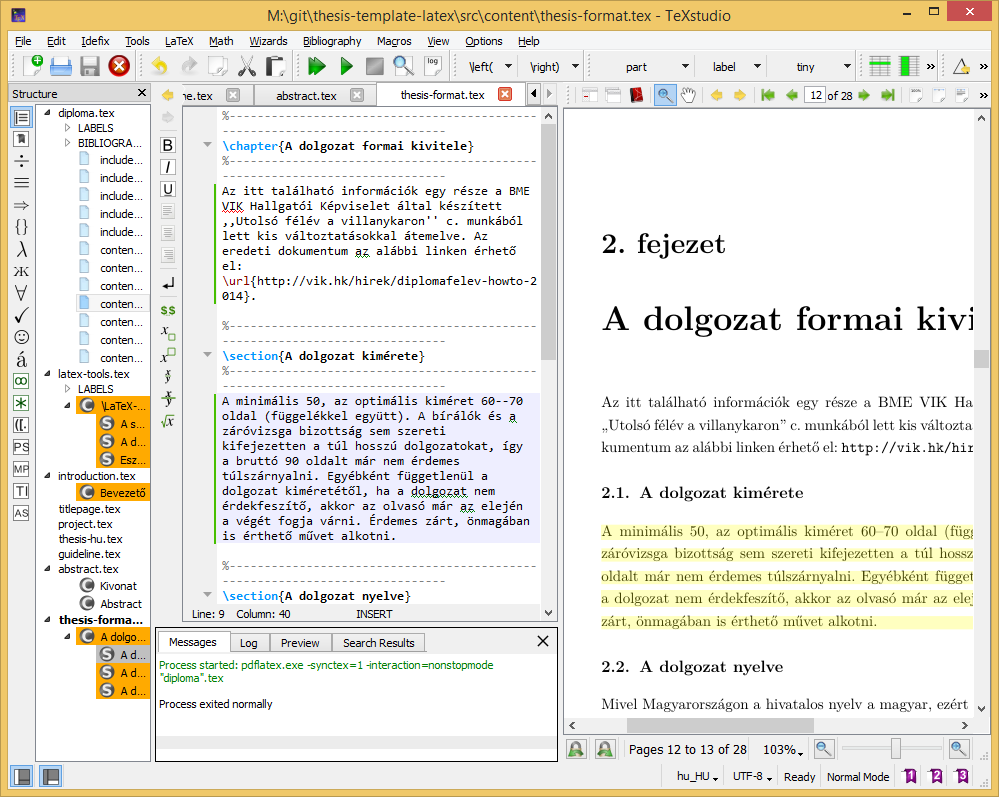
\includegraphics[width=150mm, keepaspectratio]{figures/TeXstudio.png}
\caption{A TeXstudio \LaTeX-szerkesztő.}
\label{fig:TeXstudio}
\end{figure}

A TeXstudio telepítése után érdemes még letölteni a magyar nyelvű helyesírásellenőrző-szótárakat hozzá. A TeXstudio az OpenOffice-hoz használatos formátumot tudja kezelni. A TeXstudio beállításainál a \verb+General+ fülön a \verb+Dictionaries+ résznél tudjuk megadni, hogy melyik szótárat használja.

Egy másik használható Windows alapú szerkesztőprogram a LEd\footnote{A LEd hivatalos oldala: \url{http://www.latexeditor.org/}} (LaTeX Editor), a TeXstudio azonban stabilabb, gyorsabb, és jobban használható.

%----------------------------------------------------------------------------
\subsection{A dokumentum lefordítása Windows alatt}
%----------------------------------------------------------------------------
A TeXstudio és a LEd kizárólag szerkesztőprogram (bár az utóbbiban DVI-nézegető is van), így a dokumentum fordításához szükséges eszközöket nem tartalmazza. Windows alatt alapvetően két lehetőség közül érdemes választani: MiKTeX (\url{http://miktex.org/}) és TeX Live (\url{http://www.tug.org/texlive/}) programcsomag. Az utóbbi működik Mac OS X, GNU/Linux alatt és Unix-származékokon is. A MiKTeX egy alapcsomag telepítése után mindig letölti a használt funkciókhoz szükséges, de lokálisan hiányzó \TeX-csomagokat, míg a TeX Live DVD ISO verzóban férhető hozzá. Ez a dokumentum TeX Live 2008 programcsomag segítségével fordult, amelynek DVD ISO verziója a megadott oldalról letölthető. A sablon lefordításához a disztribúcióban szereplő \verb+magyar.ldf+ fájlt a \verb+http://www.math.bme.hu/latex/+ változatra kell cserélni, vagy az utóbbi változatot be kell másolni a projekt-könyvtárba (ahogy ezt meg is tettük a sablonban) különben anomáliák tapasztalhatók a dokumentumban (pl. az ábra- és táblázat-aláírások formátuma nem a beállított lesz, vagy bizonyos oldalakon megjelenik alapértelmezésben egy fejléc). A TeX Live 2008-at még nem kell külön telepíteni a gépre, elegendő DVD-ről (vagy az ISO fájlból közvetlenül, pl. DaemonTools-szal) használni.

Ha a MiKTeX csomagot használjuk, akkor parancssorból a következő módon tudjuk újrafordítani a teljes dokumentumot:

\begin{lstlisting}[language=bash,frame=single,float=!ht]
$ texify -p thesis.tex
\end{lstlisting}

A \verb+texify+ parancs a MiKTex programcsomag \verb+miktex/bin+ alkönyvtárában található. A parancs gondoskodik arról, hogy a szükséges lépéseket (fordítás, hivatkozások generálása stb.) a megfelelő sorrendben elvégezze. A \verb+-p+ kapcsoló hatására PDF-et generál. A fordítást és az ideiglenes fájlok törlését elvégezhetjük a sablonhoz mellékelt \verb+manual_build.bat+ szkript segítségével is.

A \TeX-eszközöket tartalmazó programcsomag binárisainak elérési útját gyakran be kell állítani a szerkesztőprogramban, például TeXstudio esetén legegyszerűbben az \verb+Options / Configure TeXstudio... / Commands+ menüponttal előhívott dialógusablakban tehetjük ezt meg.

A PDF-\LaTeX~használata esetén a generált dokumentum közvetlenül PDF-formátumban áll rendelkezésre. Amennyiben a PDF-fájl egy PDF-nézőben (pl. Adobe Acrobat Reader vagy Foxit PDF Reader) meg van nyitva, akkor a fájlleírót a PDF-néző program tipikusan lefoglalja. Ilyen esetben a dokumentum újrafordítása hibaüzenettel kilép. Ha bezárjuk és újra megnyitjuk a PDF dokumentumot, akkor pedig a PDF-nézők többsége az első oldalon nyitja meg a dokumentumot, nem a legutóbb olvasott oldalon. Ezzel szemben például az egyszerű és ingyenes \textcolor{blue}{Sumatra PDF} nevű program képes arra, hogy a megnyitott dokumentum megváltozását detektálja, és frissítse a nézetet az aktuális oldal megtartásával.

%----------------------------------------------------------------------------
\subsection{Eszközök Linuxhoz}
%----------------------------------------------------------------------------
Linux operációs rendszer alatt is rengeteg szerkesztőprogram van, pl. a KDE alapú Kile jól használható. Ez ingyenesen letölthető, vagy éppenséggel az adott Linux-disztribúció eleve tartalmazza, ahogyan a dokumentum fordításához szükséges csomagokat is. Az Ubuntu Linux disztribúciók alatt például legtöbbször a \verb+texlive-*+ csomagok telepítésével használhatók a \LaTeX-eszközök. A jelen sablon fordításához szükséges csomagok (kb. 0,5 GB) az alábbi paranccsal telepíthetők:

\begin{lstlisting}[language=bash,morekeywords={sudo,apt\-get},alsoletter={-},breaklines=true]
$ sudo apt-get install texlive-latex-extra texlive-fonts-extra texlive-fonts-recommended texlive-xetex texlive-science
\end{lstlisting}

Amennyiben egy újabb csomag hozzáadása után hiányzó fájlra utaló hibát kapunk a fordítótól, telepítenünk kell az azt tartalmazó TeX Live csomagot. Ha pl. a \verb+bibentry+ csomagot szeretnénk használni, futtassuk az alábbi parancsot:

\begin{lstlisting}[language=bash,morekeywords={apt\-cache},alsoletter={-},breaklines=true]
$ apt-cache search bibentry
texlive-luatex - TeX Live: LuaTeX packages
\end{lstlisting}

Majd telepítsük fel a megfelelő TeX Live csomagot, jelen esetben a `texlive-lualatex`-et. (Egy LaTeX csomag több TeX Live csomagban is szerepelhet.)

Ha gyakran szerkesztünk más \LaTeX dokumentumokat is, kényelmes és biztos megoldás a teljes TeX Live disztribúció telepítése, ez azonban kb. 4 GB helyet igényel.

\begin{lstlisting}[language=bash,morekeywords={sudo,apt\-get},alsoletter={-},breaklines=true]
sudo apt-get install texlive-full
\end{lstlisting}

\clearpage%----------------------------------------------------------------------------
\section{A dolgozat formai kivitele}
%----------------------------------------------------------------------------
Az itt található információk egy része a BME VIK Hallgatói Képviselet által készített ,,Utolsó félév a villanykaron'' c. munkából lett kis változtatásokkal átemelve. Az eredeti dokumentum az alábbi linken érhető el: \url{http://vik.hk/hirek/diplomafelev-howto-2015}.

%----------------------------------------------------------------------------
\subsection{A dolgozat kimérete}
%----------------------------------------------------------------------------
Szakdolgozat esetében minimum 30, 45 körüli ajánlott oldalszám lehet az iránymutató. De mindenképp érdemes rákérdezni a konzulensnél is az elvárásokra, mert tanszékenként változóak lehetnek az elvárások.

Mesterképzésen a Diplomatervezés 1 esetében a beszámoló még inkább az Önálló laboratóriumi beszámolókhoz hasonlít, tanszékenként eltérő formai követelményekkel, -- egy legalább 30 oldal körüli dolgozat az elvárt -- és az elmúlt fél éves munkáról szól. De egyben célszerű, ha ez a végleges diplomaterv alapja is. (A végleges 60-90 oldal körülbelül a hasznos részre nézve)


%----------------------------------------------------------------------------
\subsection{A dolgozat nyelve}
%----------------------------------------------------------------------------
Mivel Magyarországon a hivatalos nyelv a magyar, ezért alapértelmezésben magyarul kell megírni a dolgozatot. Aki külföldi posztgraduális képzésben akar részt venni, nemzetközi szintű tudományos kutatást szeretne végezni, vagy multinacionális cégnél akar elhelyezkedni, annak célszerű angolul megírnia diplomadolgozatát. Mielőtt a hallgató az angol nyelvű verzió mellett dönt, erősen ajánlott mérlegelni, hogy ez mennyi többletmunkát fog a hallgatónak jelenteni fogalmazás és nyelvhelyesség terén, valamint -- nem utolsó sorban -- hogy ez mennyi többletmunkát fog jelenteni a konzulens illetve bíráló számára. Egy nehezen olvasható, netalán érthetetlen szöveg teher minden játékos számára.

%----------------------------------------------------------------------------
\subsection{A dokumentum nyomdatechnikai kivitele}
%----------------------------------------------------------------------------
A dolgozatot A4-es fehér lapra nyomtatva, 2,5 centiméteres margóval (+1~cm kötésbeni), 11--12 pontos betűmérettel, talpas betűtípussal és másfeles sorközzel célszerű elkészíteni.

Annak érdekében, hogy a dolgozat külsőleg is igényes munka benyomását keltse, érdemes figyelni az alapvető tipográfiai szabályok betartására~\cite{Jeney}.

\clearpage% !TeX spellcheck = hu_HU
% !TeX encoding = UTF-8
% !TeX program = xelatex
%----------------------------------------------------------------------------
\section{A \LaTeX-sablon használata}
%----------------------------------------------------------------------------

Ebben a fejezetben röviden, implicit módon bemutatjuk a sablon használatának módját, ami azt jelenti, hogy sablon használata ennek a dokumentumnak a forráskódját tanulmányozva válik teljesen világossá. Amennyiben a szoftver-keretrendszer telepítve van, a sablon alkalmazása és a dolgozat szerkesztése \LaTeX-ben a sablon segítségével tapasztalataink szerint jóval hatékonyabb, mint egy WYSWYG (\emph{What You See is What You Get}) típusú szövegszerkesztő esetén (pl. Microsoft Word, OpenOffice).

%----------------------------------------------------------------------------
\subsection{Címkék és hivatkozások}
%----------------------------------------------------------------------------
A \LaTeX~dokumentumban címkéket (\verb+\label+) rendelhetünk ábrákhoz, táblázatokhoz, fejezetekhez, listákhoz, képletekhez stb. Ezekre a dokumentum bármely részében hivatkozhatunk, a hivatkozások automatikusan feloldásra kerülnek.

A sablonban makrókat definiáltunk a hivatkozások megkönnyítéséhez. Ennek megfelelően minden ábra (\emph{figure}) címkéje \verb+fig:+ kulcsszóval kezdődik, míg minden táblázat (\emph{table}), képlet (\emph{equation}), fejezet (\emph{section}) és lista (\emph{listing}) rendre a \verb+tab:+, \verb+eq:+, \verb+sec:+ és \verb+lst:+ kulcsszóval kezdődik, és a kulcsszavak után tetszőlegesen választott címke használható. Ha ezt a konvenciót betartjuk, akkor az előbbi objektumok számára rendre a \verb+\figref+, \verb+\tabref+, \verb+\eqref+, \verb+\sectref+ és \verb+\listref+ makrókkal hivatkozhatunk. A makrók paramétere a címke, amelyre hivatkozunk (a kulcsszó nélkül). Az összes említett hivatkozástípus, beleértve az \verb+\url+ kulcsszóval bevezetett web-hivatkozásokat is a  \verb+hyperref+\footnote{Segítségével a dokumentumban megjelenő hivatkozások nem csak dinamikussá válnak, de színezhetők is, bővebbet erről a csomag dokumentációjában találunk. Ez egyúttal egy példa lábjegyzet írására.} csomagnak köszönhetően aktívak a legtöbb PDF-nézegetőben, rájuk kattintva a dokumentum megfelelő oldalára ugrik a PDF-néző vagy a megfelelő linket megnyitja az alapértelmezett böngészővel. A \verb+hyperref+ csomag a kimeneti PDF-dokumentumba könyvjelzőket is készít a tartalomjegyzékből. Ez egy szintén aktív tartalomjegyzék, amelynek elemeire kattintva a nézegető behozza a kiválasztott fejezetet.

%----------------------------------------------------------------------------
\subsection{Ábrák és táblázatok}
%----------------------------------------------------------------------------
Használjunk vektorgrafikus ábrákat, ha van rá módunk. PDFLaTeX használata esetén PDF formátumú ábrákat lehet beilleszteni könnyen, az EPS (PostScript) vektorgrafikus képformátum beillesztését a PDFLaTeX közvetlenül nem támogatja (de lehet konvertálni, lásd később). Ha vektorgrafikus formában nem áll rendelkezésünkre az ábra, akkor a  veszteségmentes PNG, valamint a veszteséges JPEG formátumban érdemes elmenteni.  Figyeljünk arra, hogy ilyenkor a képek felbontása elég nagy legyen ahhoz, hogy nyomtatásban is megfelelő minőséget nyújtson (legalább 300 dpi javasolt). A dokumentumban felhasznált képfájlokat a dokumentum forrása mellett érdemes tartani, archiválni, mivel ezek hiányában a dokumentum nem fordul újra. Ha lehet, a vektorgrafikus képeket vektorgrafikus formátumban is érdemes elmenteni az újrafelhasználhatóság (az átszerkeszthetőség) érdekében.

Kapcsolási rajzok legtöbbször kimásolhatók egy vektorgrafikus programba (pl. CorelDraw) és onnan nagyobb felbontással raszterizálva kimenthatők PNG formátumban. Ugyanakkor kiváló ábrák készíthetők Microsoft Visio vagy hasonló program használatával is: Visio-ból az ábrák közvetlenül PDF-be is menthetők.

Lehetőségeink Matlab ábrák esetén:
\begin{itemize}
	\item Képernyőlopás (\emph{screenshot}) is elfogadható minőségű lehet a dokumentumban, de általában jobb felbontást is el lehet érni más módszerrel.
	\item A Matlab ábrát a \verb+File/Save As+ opcióval lementhetjük PNG formátumban (ugyanaz itt is érvényes, mint korábban, ezért nem javasoljuk).
	\item A Matlab ábrát az \verb+Edit/Copy figure+ opcióval kimásolhatjuk egy vektorgrafikus programba is és onnan nagyobb felbontással raszterizálva kimenthatjük PNG formátumban (nem javasolt).
	\item Javasolt megoldás: az ábrát a \verb+File/Save As+ opcióval EPS \emph{vektorgrafikus} formátumban elmentjük, PDF-be konvertálva beillesztjük a dolgozatba.
\end{itemize}
Az EPS kép az \verb+epstopdf+ programmal\footnote{a korábban említett \LaTeX-disztribúciókban megtalálható} konvertálható PDF formátumba. Célszerű egy batch-fájlt készíteni az összes EPS ábra lefordítására az alábbi módon (ez Windows alatt működik).
\begin{lstlisting}[language=]
@echo off
for %%j in (*.eps) do (
  echo converting file "%%j"
  epstopdf "%%j"
)
echo done .
\end{lstlisting}

Egy ilyen parancsfájlt (\verb+convert.cmd+) elhelyeztük a sablon \verb+figures\eps+ könyvtárába, így a felhasználónak csak annyi a dolga, hogy a \verb+figures\eps+ könyvtárba kimenti az EPS formátumú vektorgrafikus képet, majd lefuttatja a \verb+convert.cmd+ parancsfájlt, ami PDF-be konvertálja az EPS fájlt.

Ezek után a PDF-ábrát ugyanúgy lehet a dokumentumba beilleszteni, mint a PNG-t vagy a JPEG-et. A megoldás előnye, hogy a lefordított dokumentumban is vektorgrafikusan tárolódik az ábra, így a mérete jóval kisebb, mintha raszterizáltuk volna beillesztés előtt. Ez a módszer minden -- az EPS formátumot ismerő -- vektorgrafikus program (pl. CorelDraw) esetén is használható.

A képek beillesztésére \az+\refstruc{sec:LatexTools}ben mutattunk be példát (\refstruc{fig:TeXstudio}). Az előző mondatban egyúttal az automatikusan feloldódó ábrahivatkozásra is láthatunk példát. Több képfájlt is beilleszthetünk egyetlen ábrába. Az egyes képek közötti horizontális és vertikális margót metrikusan szabályozhatjuk (\refstruc{fig:HVSpaces}). Az ábrák elhelyezését számtalan tipográfiai szabály egyidejű teljesítésével a fordító maga végzi, a dokumentum írója csak preferenciáit jelezheti a fordító felé (olykor ez bosszúságot is okozhat, ilyenkor pl. a kép méretével lehet játszani).

\begin{figure}[!ht]
	\centering
	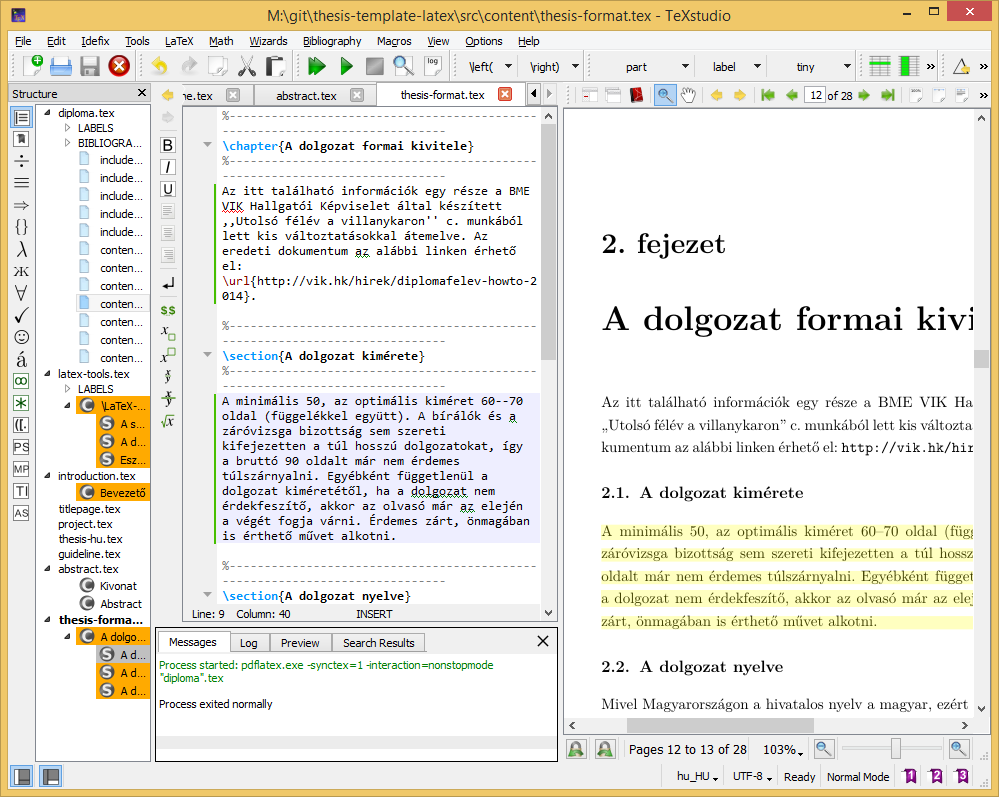
\includegraphics[width=67mm, keepaspectratio]{figures/TeXstudio.png}\hspace{1cm}
	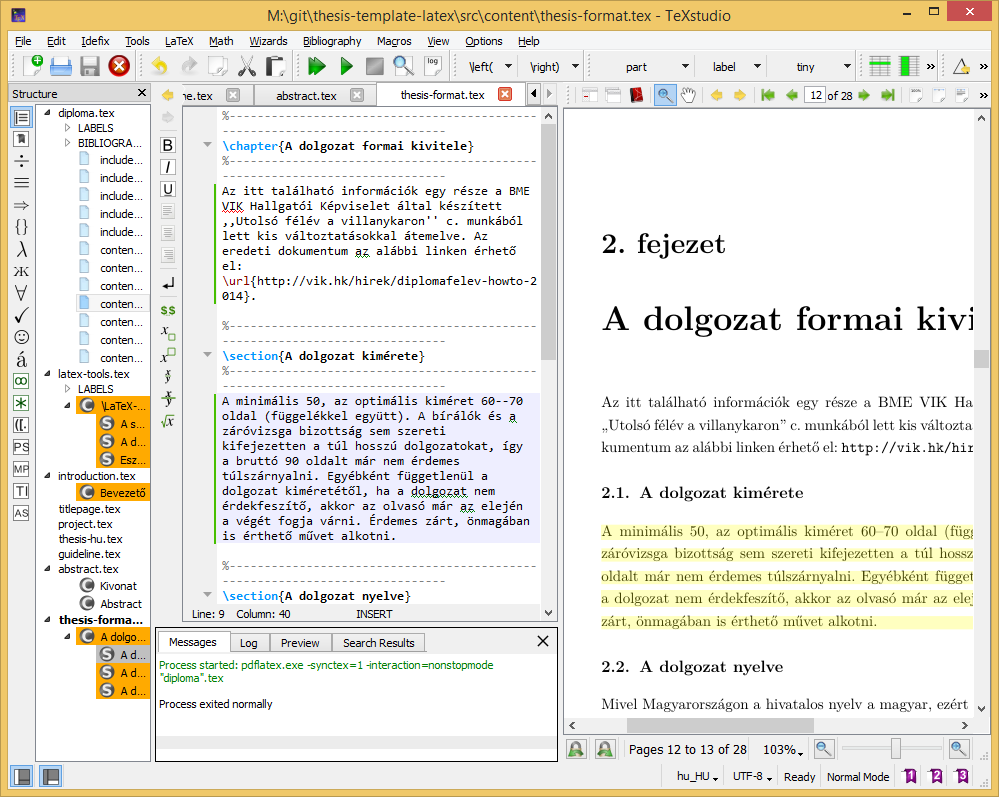
\includegraphics[width=67mm, keepaspectratio]{figures/TeXstudio.png}\\\vspace{5mm}
	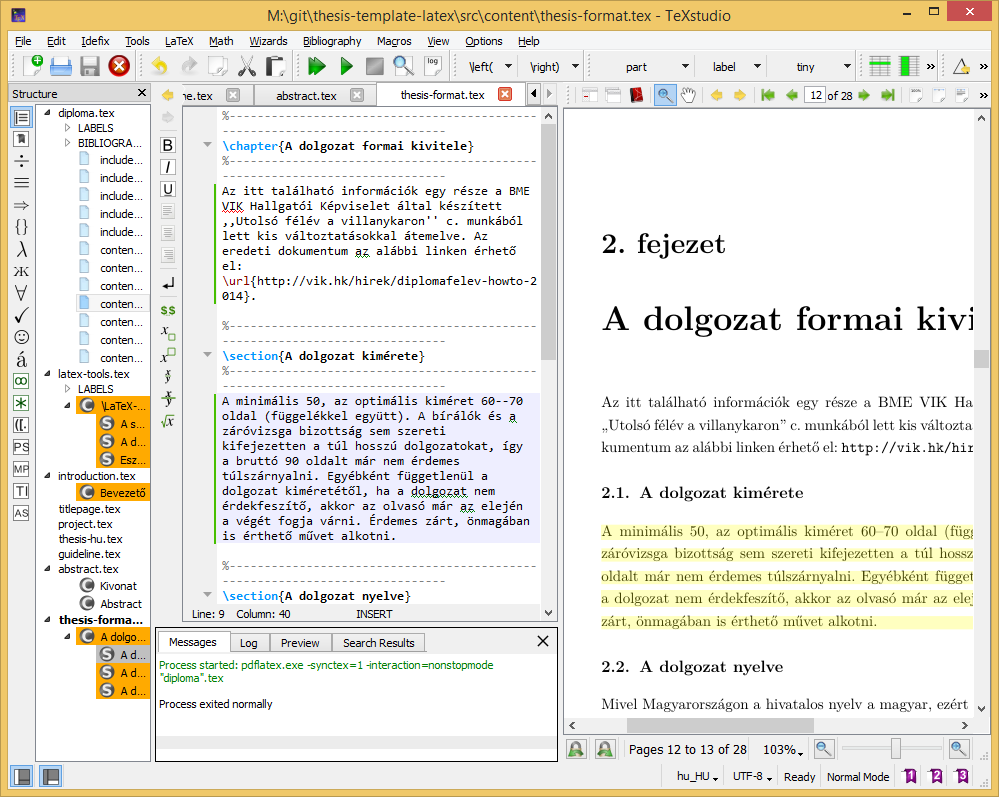
\includegraphics[width=67mm, keepaspectratio]{figures/TeXstudio.png}\hspace{1cm}
	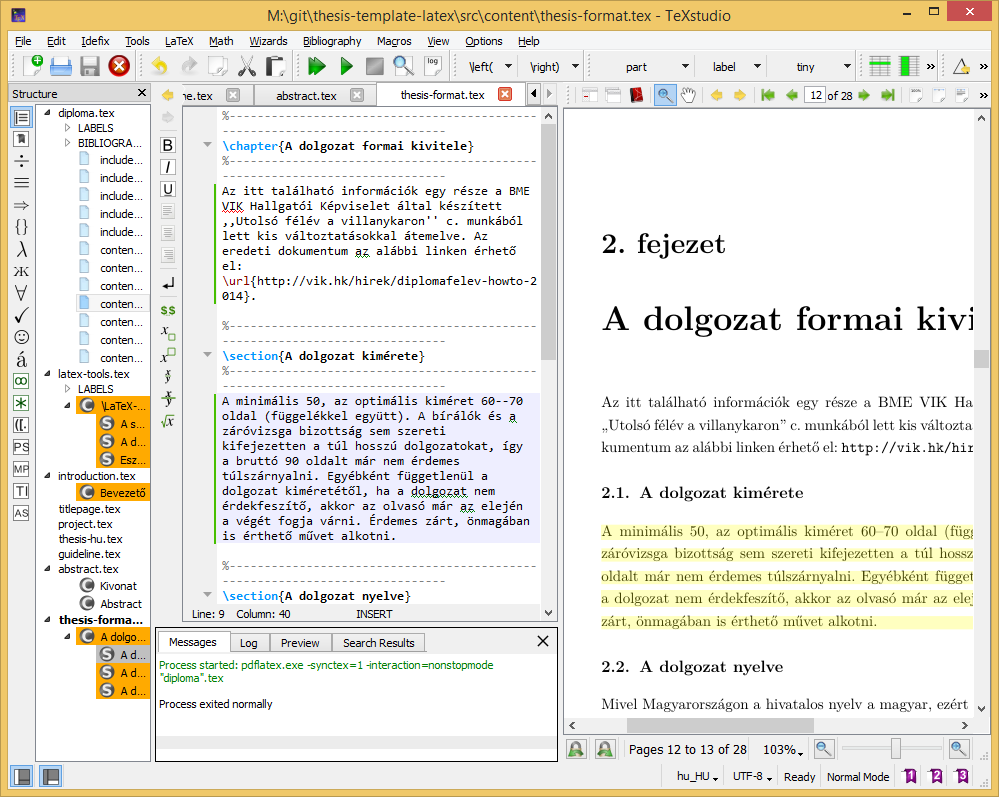
\includegraphics[width=67mm, keepaspectratio]{figures/TeXstudio.png}
	\caption{Több képfájl beillesztése esetén térközöket is érdemes használni.}
	\label{fig:HVSpaces}
\end{figure}

A táblázatok használatára \aref{tab:TabularExample}~táblázat mutat példát. A táblázatok formázásához hasznos tanácsokat találunk a \verb+booktabs+ csomag dokumentációjában.

\begin{table}[ht]
	\footnotesize
	\centering
	\begin{tabular}{ l c c }
		\toprule
		Órajel & Frekvencia & Cél pin \\
		\midrule
		CLKA & 100 MHz & FPGA CLK0\\
		CLKB & 48 MHz  & FPGA CLK1\\
		CLKC & 20 MHz  & Processzor\\
		CLKD & 25 MHz  & Ethernet chip \\
		CLKE & 72 MHz  & FPGA CLK2\\
		XBUF & 20 MHz  & FPGA CLK3\\
		\bottomrule
	\end{tabular}
	\caption{Az órajel-generátor chip órajel-kimenetei.}
	\label{tab:TabularExample}
\end{table}


%----------------------------------------------------------------------------
\subsection{Felsorolások és listák}
%----------------------------------------------------------------------------
Számozatlan felsorolásra mutat példát a jelenlegi bekezdés:
\begin{itemize}
	\item \emph{első bajusz:} ide lehetne írni az első elem kifejését,
	\item \emph{második bajusz:} ide lehetne írni a második elem kifejését,
	\item \emph{ez meg egy szakáll:} ide lehetne írni a harmadik elem kifejését.
\end{itemize}

Számozott felsorolást is készíthetünk az alábbi módon:
\begin{enumerate}
	\item \emph{első bajusz:} ide lehetne írni az első elem kifejését, és ez a kifejtés így néz ki, ha több sorosra sikeredik,
	\item \emph{második bajusz:} ide lehetne írni a második elem kifejését,
	\item \emph{ez meg egy szakáll:} ide lehetne írni a harmadik elem kifejését.
\end{enumerate}
A felsorolásokban sorok végén vessző, az utolsó sor végén pedig pont a szokásos írásjel. Ez alól kivételt képezhet, ha az egyes elemek több teljes mondatot tartalmaznak.

Listákban a dolgozat szövegétől elkülönítendő kódrészleteket, programsorokat, pszeudo-kódokat jeleníthetünk meg (\ref{lst:Example}.~kódrészlet).
\begin{lstlisting}[language=tex,caption=A fenti számozott felsorolás \LaTeX-forráskódja,label=lst:Example]
\begin{enumerate}
	\item \emph{els(*@ő@*) bajusz:} ide lehetne írni az els(*@ő@*) elem kifejését,
	és ez a kifejtés így néz ki, ha több sorosra sikeredik,
	\item \emph{második bajusz:} ide lehetne írni a második elem kifejését,
	\item \emph{ez meg egy szakáll:} ide lehetne írni a harmadik elem kifejését.
\end{enumerate}
\end{lstlisting}
A lista keretét, háttérszínét, egész stílusát megválaszthatjuk. Ráadásul különféle programnyelveket és a nyelveken belül kulcsszavakat is definiálhatunk, ha szükséges. Erről bővebbet a \verb+listings+ csomag hivatalos leírásában találhatunk.

%----------------------------------------------------------------------------
\subsection{Képletek}
%----------------------------------------------------------------------------
Ha egy formula nem túlságosan hosszú, és nem akarjuk hivatkozni a szövegből, mint például a $e^{i\pi}+1=0$ képlet, \emph{szövegközi képletként} szokás leírni. Csak, hogy másik példát is lássunk, az $U_i=-d\Phi/dt$ Faraday-törvény a $\rot E=-\frac{dB}{dt}$ differenciális alakban adott Maxwell-egyenlet felületre vett integráljából vezethető le. Látható, hogy a \LaTeX-fordító a sorközöket betartja, így a szöveg szedése esztétikus marad szövegközi képletek használata esetén is.

Képletek esetén az általános konvenció, hogy a kisbetűk skalárt, a kis félkövér betűk ($\mathbf{v}$) oszlopvektort -- és ennek megfelelően $\mathbf{v}^T$ sorvektort -- a kapitális félkövér betűk ($\mathbf{V}$) mátrixot jelölnek. Ha ettől el szeretnénk térni, akkor az alkalmazni kívánt jelölésmódot célszerű külön alfejezetben definiálni. Ennek megfelelően, amennyiben $\mathbf{y}$ jelöli a mérések vektorát, $\mathbf{\vartheta}$ a paraméterek vektorát és $\hat{\mathbf{y}}=\mathbf{X}\vartheta$ a paraméterekben lineáris modellt, akkor a \emph{Least-Squares} értelemben optimális paraméterbecslő $\hat{\mathbf{\vartheta}}_{LS}=(\mathbf{X}^T\mathbf{X})^{-1}\mathbf{X}^T\mathbf{y}$ lesz.

Emellett kiemelt, sorszámozott képleteket is megadhatunk, ennél az \verb+equation+ és a \verb+eqnarray+ környezetek helyett a korszerűbb \verb+align+ környezet alkalmazását javasoljuk (több okból, különféle problémák elkerülése végett, amelyekre most nem térünk ki). Tehát
\begin{align}
\dot{\mathbf{x}}&=\mathbf{A}\mathbf{x}+\mathbf{B}\mathbf{u},\\
\mathbf{y}&=\mathbf{C}\mathbf{x},
\end{align}
ahol $\mathbf{x}$ az állapotvektor, $\mathbf{y}$ a mérések vektora és $\mathbf{A}$, $\mathbf{B}$ és $\mathbf{C}$ a rendszert leíró paramétermátrixok. Figyeljük meg, hogy a két egyenletben az egyenlőségjelek egymáshoz igazítva jelennek meg, mivel a mindkettőt az \& karakter előzi meg a kódban. Lehetőség van számozatlan kiemelt képlet használatára is, például
\begin{align}
\dot{\mathbf{x}}&=\mathbf{A}\mathbf{x}+\mathbf{B}\mathbf{u},\nonumber\\
\mathbf{y}&=\mathbf{C}\mathbf{x}\nonumber.
\end{align}
Mátrixok felírására az $\mathbf{A}\mathbf{x}=\mathbf{b}$ inhomogén lineáris egyenlet részletes kifejtésével mutatunk példát:
\begin{align}
\begin{bmatrix}
a_{11} & a_{12} & \dots & a_{1n}\\
a_{21} & a_{22} & \dots & a_{2n}\\
\vdots & \vdots & \ddots & \vdots\\
a_{m1} & a_{m2} & \dots & a_{mn}
\end{bmatrix}
\begin{pmatrix}x_1\\x_2\\\vdots\\x_n\end{pmatrix}=
\begin{pmatrix}b_1\\b_2\\\vdots\\b_m\end{pmatrix}.
\end{align}
A \verb+\frac+ utasítás hatékonyságát egy általános másodfokú tag átviteli függvényén keresztül mutatjuk be, azaz
\begin{align}
W(s)=\frac{A}{1+2T\xi s+s^2T^2}.
\end{align}
A matematikai mód minden szimbólumának és képességének a bemutatására természetesen itt nincs lehetőség, de gyors referenciaként hatékonyan használhatók a következő linkek:\\
\indent\url{http://www.artofproblemsolving.com/LaTeX/AoPS_L_GuideSym.php},\\
\indent\url{http://www.ctan.org/tex-archive/info/symbols/comprehensive/symbols-a4.pdf},\\
\indent\url{ftp://ftp.ams.org/pub/tex/doc/amsmath/short-math-guide.pdf}.\\
Ez pedig itt egy magyarázat, hogy miért érdemes \verb+align+ környezetet használni:\\
\indent\url{http://texblog.net/latex-archive/maths/eqnarray-align-environment/}.

%----------------------------------------------------------------------------
\subsection{Irodalmi hivatkozások}
\label{sec:HowtoReference}
%----------------------------------------------------------------------------
Egy \LaTeX~dokumentumban az irodalmi hivatkozások definíciójának két módja van. Az egyik a \verb+\thebibliograhy+ környezet használata a dokumentum végén, az \verb+\end{document}+ lezárás előtt.
\begin{lstlisting}[language=tex]
\begin{thebibliography}{9}

\bibitem{Lamport94} Leslie Lamport, \emph{\LaTeX: A Document Preparation System}.
Addison Wesley, Massachusetts, 2nd Edition, 1994.

\end{thebibliography}
\end{lstlisting}

Ezek után a dokumentumban a \verb+\cite{Lamport94}+ utasítással hivatkozhatunk a forrásra. A fenti megadás viszonylag kötetlen, a szerző maga formázza az irodalomjegyzéket (ami gyakran inkonzisztens eredményhez vezet).

Egy sokkal professzionálisabb módszer a BiB\TeX{} használata, ezért ez a sablon is ezt támogatja. Ebben az esetben egy külön szöveges adatbázisban definiáljuk a forrásmunkákat, és egy külön stílusfájl határozza meg az irodalomjegyzék kinézetét. Ez, összhangban azzal, hogy külön formátumkonvenció határozza meg a folyóirat-, a könyv-, a konferenciacikk- stb. hivatkozások kinézetét az irodalomjegyzékben (a sablon használata esetén ezzel nem is kell foglalkoznia a hallgatónak, de az eredményt célszerű ellenőrizni). felhasznált hivatkozások adatbázisa egy \verb+.bib+ kiterjesztésű szöveges fájl, amelynek szerkezetét a \Aref{lst:Bibtex} kódrészlet demonstrálja. A forrásmunkák bevitelekor a sor végi vesszők külön figyelmet igényelnek, mert hiányuk a BiB\TeX-fordító hibaüzenetét eredményezi. A forrásmunkákat típus szerinti kulcsszó vezeti be (\verb+@book+ könyv, \verb+@inproceedings+ konferenciakiadványban megjelent cikk, \verb+@article+ folyóiratban megjelent cikk, \verb+@techreport+ valamelyik egyetem gondozásában megjelent műszaki tanulmány, \verb+@manual+ műszaki dokumentáció esetén stb.). Nemcsak a megjelenés stílusa, de a kötelezően megadandó mezők is típusról-típusra változnak. Egy jól használható referencia a \url{http://en.wikipedia.org/wiki/BibTeX} oldalon található.

\begin{lstlisting}[caption=Példa szöveges irodalomjegyzék-adatbázisra Bib\TeX{} használata esetén.,label=lst:Bibtex]
@book{Wettl04,
  author    = {Ferenc Wettl and Gyula Mayer and Péter Szabó},
  publisher = {Panem Könyvkiadó},
  title     = {\LaTeX~kézikönyv},
  year      = {2004},
}

@article{Candy86,
  author       = {James C. Candy},
  journaltitle = {{IEEE} Trans.\ on Communications},
  month        = {01},
  note         = {\doi{10.1109/TCOM.1986.1096432}},
  number       = {1},
  pages        = {72--76},
  title        = {Decimation for Sigma Delta Modulation},
  volume       = {34},
  year         = {1986},
}

@inproceedings{Lee87,
  author    = {Wai L. Lee and Charles G. Sodini},
  booktitle = {Proc.\ of the IEEE International Symposium on Circuits and Systems},
  location  = {Philadelphia, PA, USA},
  month     = {05~4--7},
  pages     = {459--462},
  title     = {A Topology for Higher Order Interpolative Coders},
  vol       = {2},
  year      = {1987},
}

@thesis{KissPhD,
  author      = {Peter Kiss},
  institution = {Technical University of Timi\c{s}oara, Romania},
  month       = {04},
  title       = {Adaptive Digital Compensation of Analog Circuit Imperfections for Cascaded Delta-Sigma Analog-to-Digital Converters},
  type        = {phdthesis},
  year        = {2000},
}

@manual{Schreier00,
  author       = {Richard Schreier},
  month        = {01},
  note         = {\url{http://www.mathworks.com/matlabcentral/fileexchange/}},
  organization = {Oregon State University},
  title        = {The Delta-Sigma Toolbox v5.2},
  year         = {2000},
}

@misc{DipPortal,
  author       = {{Budapesti Műszaki és Gazdaságtudományi Egyetem Villamosmérnöki és Informatikai Kar}},
  howpublished = {\url{http://diplomaterv.vik.bme.hu/}},
  title        = {Diplomaterv portál (2011. február 26.)},
}

@incollection{Mkrtychev:1997,
  author    = {Mkrtychev, Alexey},
  booktitle = {Logical Foundations of Computer Science},
  doi       = {10.1007/3-540-63045-7_27},
  editor    = {Adian, Sergei and Nerode, Anil},
  isbn      = {978-3-540-63045-6},
  pages     = {266-275},
  publisher = {Springer Berlin Heidelberg},
  series    = {Lecture Notes in Computer Science},
  title     = {Models for the logic of proofs},
  url       = {http://dx.doi.org/10.1007/3-540-63045-7_27},
  volume    = {1234},
  year      = {1997},
}
\end{lstlisting}

A stílusfájl egy \verb+.sty+ kiterjesztésű fájl, de ezzel lényegében nem kell foglalkozni, mert vannak beépített stílusok, amelyek jól használhatók. Ez a sablon a BiB\TeX-et használja, a hozzá tartozó adatbázisfájl a \verb+mybib.bib+ fájl. Megfigyelhető, hogy az irodalomjegyzéket a dokumentum végére (a \verb+\end{document}+ utasítás elé) beillesztett \verb+\bibliography{mybib}+ utasítással hozhatjuk létre, a stílusát pedig ugyanitt a  \verb+\bibliographystyle{plain}+ utasítással adhatjuk meg. Ebben az esetben a \verb+plain+ előre definiált stílust használjuk (a sablonban is ezt állítottuk be). A \verb+plain+ stíluson kívül természetesen számtalan más előre definiált stílus is létezik. Mivel a \verb+.bib+ adatbázisban ezeket megadtuk, a BiB\TeX-fordító is meg tudja különböztetni a szerzőt a címtől és a kiadótól, és ez alapján automatikusan generálódik az irodalomjegyzék a stílusfájl által meghatározott stílusban.

Az egyes forrásmunkákra a szövegből továbbra is a \verb+\cite+ paranccsal tudunk hivatkozni, így \aref{lst:Bibtex}.~kódrészlet esetén a hivatkozások a \verb+\cite+ parancs paraméterével rendre \texttt{Wettl04}, \texttt{Candy86}, \texttt{Lee87}, \texttt{KissPhD}, \texttt{Schreirer00}, \texttt{Mkrtychev:1997} és \texttt{DipPortal}. Az egyes forrásmunkák sorszáma az irodalomjegyzék bővítésekor változhat. Amennyiben az aktuális számhoz illeszkedő névelőt szeretnénk használni, használjuk az \verb+\acite{}+ parancsot.

Az irodalomjegyzékben alapértelmezésben csak azok a forrásmunkák jelennek meg, amelyekre található hivatkozás a szövegben, és ez így alapvetően helyes is, hiszen olyan forrásmunkákat nem illik az irodalomjegyzékbe írni, amelyekre nincs hivatkozás.

Mivel a fordítási folyamat során több lépésben oldódnak fel a szimbólumok, ezért gyakran többször is le kell fordítani a dokumentumot. Ilyenkor ez első 1-2 fordítás esetleg szimbólum-feloldásra vonatkozó figyelmeztető üzenettel zárul. Ha hibaüzenettel zárul bármelyik fordítás, akkor nincs értelme megismételni, hanem a hibát kell megkeresni. A \verb+.bib+ fájl megváltoztatáskor sokszor nincs hatása a változtatásnak azonnal, mivel nem mindig fut újra a BibTeX fordító. Ezért célszerű a változtatás után azt manuálisan is lefuttatni (TeXstudio esetén \verb+Tools/Bibliography+).

Hogy a szövegbe ágyazott hivatkozások kinézetét demonstráljuk, itt most sorban meghivatkozzuk a \cite{Wettl04}, \cite{Candy86}, \cite{Lee87}, \cite{KissPhD}, \cite{Schreier00} és \acite{Mkrtychev:1997}\footnote{Informatikai témában gyakran hivatkozunk cikkeket a Springer LNCS valamely kötetéből, ez a hivatkozás erre mutat egy helyes példát.} forrásmunkát, valamint \acite{DipPortal} weboldalt.

Megjegyzendő, hogy az ékezetes magyar betűket is tartalmazó \verb+.bib+ fájl az \verb+inputenc+ csomaggal betöltött \verb+latin2+ betűkészlet miatt fordítható. Ugyanez a \verb+.bib+ fájl hibaüzenettel fordul egy olyan dokumentumban, ami nem tartalmazza a \verb+\usepackage[latin2]{inputenc}+ sort. Speciális igény esetén az irodalmi adatbázis általánosabb érvényűvé tehető, ha az ékezetes betűket speciális latex karakterekkel helyettesítjük a \verb+.bib+ fájlban, pl. á helyett \verb+\'{a}+-t vagy ő helyett \verb+\H{o}+-t írunk.

Irodalomhivatkozásokat célszerű először olyan szolgáltatásokban keresni, ahol jó minőségű bejegyzések találhatók (pl. ACM Digital Library,\footnote{\url{https://dl.acm.org/}} DBLP,\footnote{\url{http://dblp.uni-trier.de/}} IEEE Xplore,\footnote{\url{http://ieeexplore.ieee.org/}} SpringerLink\footnote{\url{https://link.springer.com/}}) és csak ezek után használni kevésbé válogatott forrásokat (pl. Google Scholar\footnote{\url{http://scholar.google.com/}}). A jó minőségű bejegyzéseket is érdemes megfelelően tisztítani.\footnote{\url{https://github.com/FTSRG/cheat-sheets/wiki/BibTeX-Fixing-entries-from-common-sources}} A sablon angol nyelvű változatában használt \texttt{plainnat} beállítás egyik sajátossága, hogy a cikkhez generált hivatkozás a cikk DOI-ját és URL-jét is tartalmazza, ami gyakran duplikátumhoz vezet -- érdemes tehát a DOI-kat tartalmazó URL mezőket törölni. 

%----------------------------------------------------------------------------
\subsection{A dolgozat szerkezete és a forrásfájlok}
%----------------------------------------------------------------------------
A diplomatervsablonban a TeX fájlok két alkönyvtárban helyezkednek el. Az \verb+include+ könyvtárban azok szerepelnek, amiket tipikusan nem kell szerkesztenünk, ezek a sablon részei (pl. címoldal). A \verb+content+ alkönyvtárban pedig a saját munkánkat helyezhetjük el. Itt érdemes az egyes fejezeteket külön \TeX{} állományokba rakni.

A diplomatervsablon (a kari irányelvek szerint) az alábbi fő fejezetekből áll:
\begin{enumerate}
	\item 1 oldalas \emph{tájékoztató} a szakdolgozat/diplomaterv szerkezetéről (\verb+include/guideline.tex+), ami a végső dolgozatból törlendő,
	\item \emph{feladatkiírás} (\verb+include/project.tex+), a dolgozat nyomtatott verzójában ennek a helyére kerül a tanszék által kiadott, a tanszékvezető által aláírt feladatkiírás, a dolgozat elektronikus verziójába pedig a feladatkiírás egyáltalán ne kerüljön bele, azt külön tölti fel a tanszék a diplomaterv-honlapra,
	\item \emph{címoldal} (\verb+include/titlepage.tex+),
	\item \emph{tartalomjegyzék} (\verb+thesis.tex+),
	\item a diplomatervező \emph{nyilatkozat}a az önálló munkáról (\verb+include/declaration.tex+),
	\item 1-2 oldalas tartalmi \emph{összefoglaló} magyarul és angolul, illetve elkészíthető még további nyelveken is (\verb+content/abstract.tex+),
	\item \emph{bevezetés}: a feladat értelmezése, a tervezés célja, a feladat indokoltsága, a diplomaterv felépítésének rövid összefoglalása (\verb+content/introduction.tex+),
	\item sorszámmal ellátott \emph{fejezetek}: a feladatkiírás pontosítása és részletes elemzése, előzmények (irodalomkutatás, hasonló alkotások), az ezekből levonható következtetések, a tervezés részletes leírása, a döntési lehetőségek értékelése és a választott megoldások indoklása, a megtervezett műszaki alkotás értékelése, kritikai elemzése, továbbfejlesztési lehetőségek,
	\item esetleges \emph{köszönetnyilvánítás}ok (\verb+content/acknowledgement.tex+),
	\item részletes és pontos \emph{irodalomjegyzék} (ez a sablon esetében automatikusan generálódik a \verb+thesis.tex+ fájlban elhelyezett \verb+\bibliography+ utasítás hatására, \az+\refstruc{sec:HowtoReference}ban leírtak szerint),
	\item \emph{függelékek} (\verb+content/appendices.tex+).
\end{enumerate}

A sablonban a fejezetek a \verb+thesis.tex+ fájlba vannak beillesztve \verb+\include+ utasítások segítségével. Lehetőség van arra, hogy csak az éppen szerkesztés alatt álló \verb+.tex+ fájlt fordítsuk le, ezzel lerövidítve a fordítási folyamatot. Ezt a lehetőséget az alábbi kódrészlet biztosítja a \verb+thesis.tex+ fájlban.
\begin{lstlisting}
\includeonly{
	guideline,%
	project,%
	titlepage,%
	declaration,%
	abstract,%
	introduction,%
	chapter1,%
	chapter2,%
	chapter3,%
	acknowledgement,%
	appendices,%
}
\end{lstlisting}

Ha az alábbi kódrészletben az egyes sorokat a \verb+%+ szimbólummal kikommentezzük, akkor a megfelelő \verb+.tex+ fájl nem fordul le. Az oldalszámok és a tartalomjegyék természetesen csak akkor billennek helyre, ha a teljes dokumentumot lefordítjuk.

%----------------------------------------------------------------------------
\newpage
\subsection{Alapadatok megadása}
%----------------------------------------------------------------------------
A diplomaterv alapadatait (cím, szerző, konzulens, konzulens titulusa) a \verb+thesis.tex+ fájlban lehet megadni.

%----------------------------------------------------------------------------
\subsection{Új fejezet írása}
%----------------------------------------------------------------------------
A főfejezetek külön \verb+content+ könyvtárban foglalnak helyet. A sablonhoz 3 fejezet készült. További főfejezeteket úgy hozhatunk létre, ha új \TeX~fájlt készítünk a fejezet számára, és a \verb+thesis.tex+ fájlban, a \verb+\include+ és \verb+\includeonly+ utasítások argumentumába felvesszük az új \verb+.tex+ fájl nevét.


%----------------------------------------------------------------------------
\subsection{Definíciók, tételek, példák}
%----------------------------------------------------------------------------

\begin{definition}[Fluxuskondenzátor térerőssége]
Lorem ipsum dolor sit amet, consectetur adipiscing elit, sed do eiusmod tempor incididunt ut labore et dolore magna aliqua. Ut enim ad minim veniam, quis nostrud exercitation ullamco laboris nisi ut aliquip ex ea commodo consequat.
\end{definition}

\begin{example}
Példa egy példára. Duis aute irure dolor in reprehenderit in voluptate velit esse cillum dolore eu fugiat nulla pariatur. Excepteur sint occaecat cupidatat non proident, sunt in culpa qui officia deserunt mollit anim id est laborum.
\end{example}

\begin{theorem}[Kovács tétele]
Duis aute irure dolor in reprehenderit in voluptate velit esse cillum dolore eu fugiat nulla pariatur. Excepteur sint occaecat cupidatat non proident, sunt in culpa qui officia deserunt mollit anim id est laborum.
\end{theorem}

\clearpage%----------------------------------------------------------------------------
\section{Példák a BME-sablonból}
\subsection{A TeXstudio felülete}
%----------------------------------------------------------------------------
\begin{figure}[!ht]
\centering
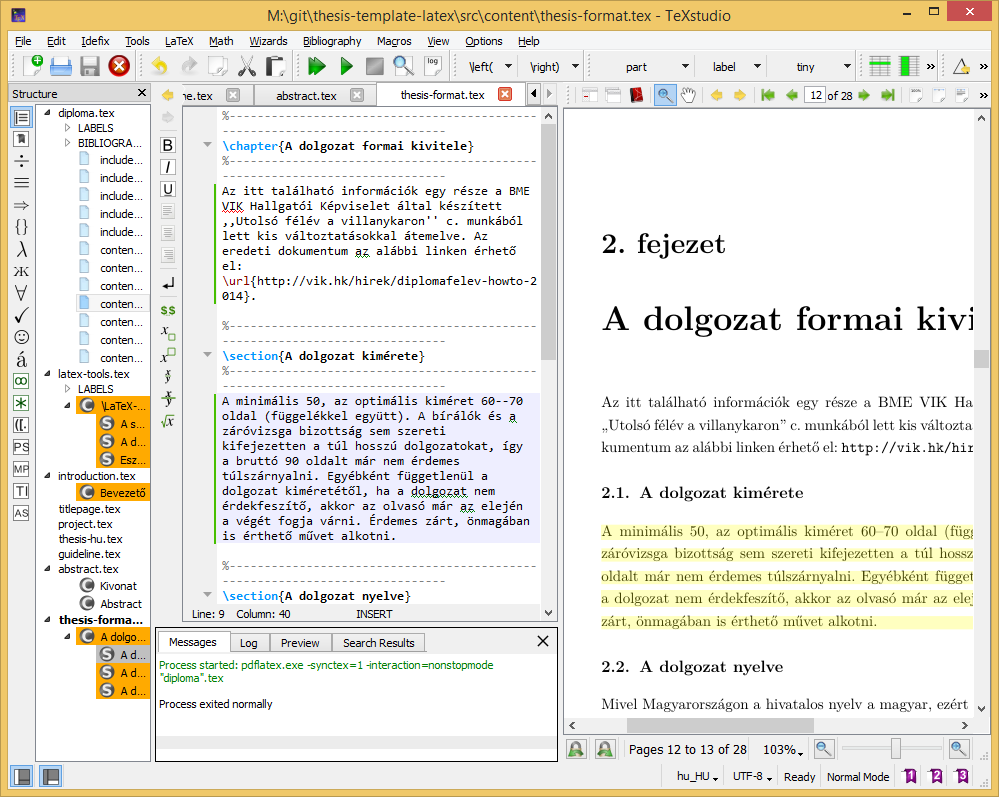
\includegraphics[width=150mm, keepaspectratio]{figures/TeXstudio.png}
\caption{A TeXstudio \LaTeX-szerkesztő.} 
\end{figure}

%----------------------------------------------------------------------------
\clearpage\subsection{Válasz az ,,Élet, a világmindenség, meg minden'' kérdésére}
%----------------------------------------------------------------------------
A Pitagorasz-tételből levezetve
\begin{align}
c^2=a^2+b^2=42.
\end{align}
A Faraday-indukciós törvényből levezetve
\begin{align}
\rot E=-\frac{dB}{dt}\hspace{1cm}\longrightarrow \hspace{1cm}
U_i=\oint\limits_\mathbf{L}{\mathbf{E}\mathbf{dl}}=-\frac{d}{dt}\int\limits_A{\mathbf{B}\mathbf{da}}=42.
\end{align}

\selectthesislanguage
